\documentclass{article}

\usepackage{graphicx}
\usepackage{amsmath}
\usepackage{amssymb}
\usepackage{courier}
\usepackage{float}
\usepackage{booktabs}
\usepackage{array}
\usepackage{enumitem}
\usepackage{tabularx}

\begin{document}

\begin{titlepage}
\begin{center}


{\huge \textbf{COS 710: Assignment III}}

\vspace{1cm}

{\Large \textbf{Structure-Based Genetic Programming}}

\vspace{1cm}

{\large u22498037 \\
University of Pretoria}


\vfill

\end{center}
\end{titlepage}

\tableofcontents

\newpage

\section{Running Instructions}
To run the GP, made with C++, a \texttt{makefile} is included as part of the submission. The following commands in the directory can be used to run the GP:

\begin{verbatim}
  make
  make run
\end{verbatim}

Since architectures may vary, the following can be commands can also be used to (hopefully) run the GP when \texttt{clang} is installed:

\begin{verbatim}
  make alt
  make run
\end{verbatim}

Running this on a Macbook Air M1 with 16GB RAM averaged 84.53 seconds per structure-based GP run and 54.59 seconds per normal GP run. There is no need to run the preprocessing script again.

\section{Notation}
The following abbreviations is used for the remainder of this report:
\begin{enumerate}
  \item \textbf{SBGP:} Structure-based Genetic Programming
  \item \textbf{NGP:} Normal Genetic Programming
\end{enumerate}

\section{Exploratory Data Analysis (EDA)}
\label{EDA}
To understand the data, Exploratory Data Analysis (EDA) were done to understand the relationship between the different datasets to discover any inconsistencies. In Section \ref{preprocessing}, the dataset will be processed based on the EDA.

It was evident that the target variable is imbalanced (Figure \ref{allDist}, bottom right) where \texttt{1.0} is live and \texttt{0.0} is die. This impacted the fitness function described in Section \ref{fitness}. Other variables such as sex, antivirals, and anorexia can also considered to be skewed (Figure \ref{allDist}). 

\begin{figure}[H]
  \makebox[\textwidth][c]{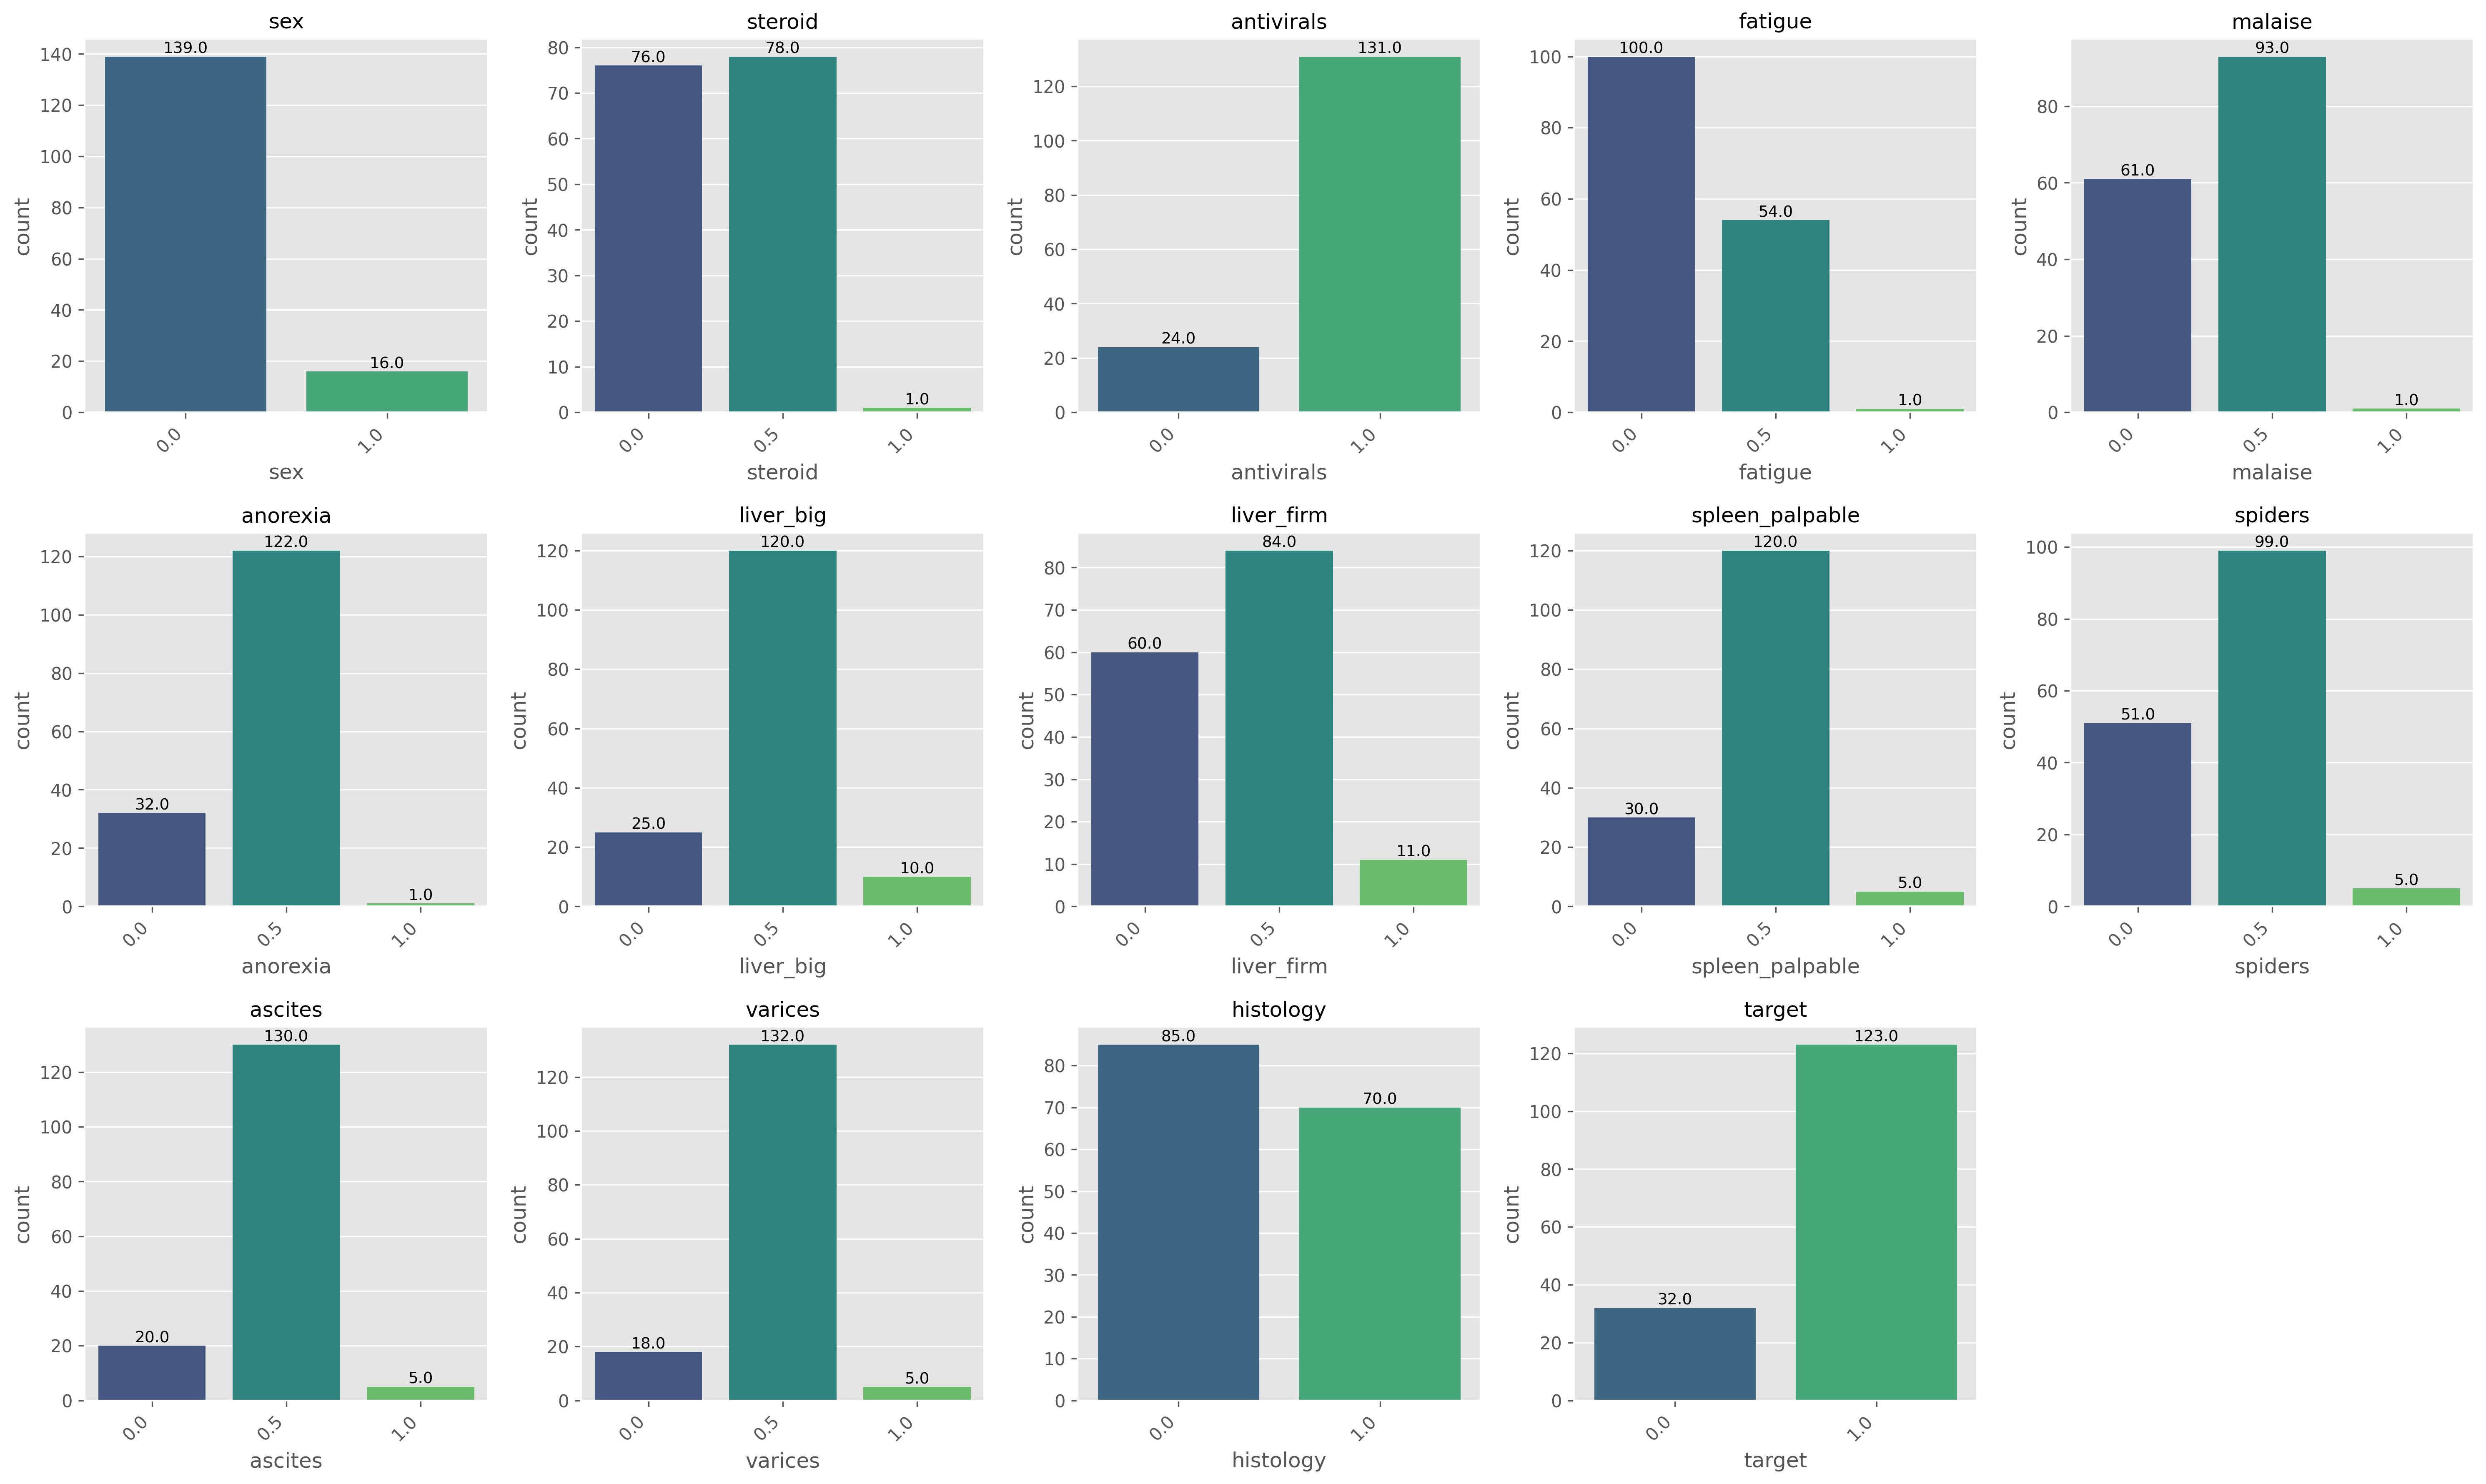
\includegraphics[width=1.5\textwidth]{../preprocessing/categorical_distributions.png}}
  \caption{A histogram visualising the distribution of all the features.}
  \label{allDist}
\end{figure}

\section{Preprocessing}
\label{preprocessing}
\subsection{Duplicates}
No duplicates were detected and therefore no further action were taken in this regard.

\subsection{Outliers}
To remove the outlier entries, data points with a \(\pm{3}\) \(Z\)-score (an indication of how many standard deviations the point is away from the mean) were removed. Removing outliers helped the model to converge better due to more consistent tree outputs. Since only one row were removed, it didn't greatly impact the model's ability to convergence, but the outlier were removed regardless of the outcome.

\subsection{Skewness}
As noted in Section \ref{EDA}, a few of the variables, including the target variable, were skewed. No further preprocessing was done with regards to skewness as the fitness function (described in Section \ref{fitness}) catered for the imbalanced data.

Experiments were conducted by upsampling the target variable to balance the dataset, but it caused the rest of the features to lose meaning when training.

\subsection{Column-wise Min-Max Normalisation}
The data was normalised column-wise using min-max scaling \cite{patro_2015_normalization}:
\begin{equation}\label{norm}
  X' = \frac{X-min}{max-min}
\end{equation}
This helped to preserve each column's features and its respective scale. Although \(tanh\), the fitness function, resides in the range \((-1,1)\), it was still essential to scale the dataset to be on the same scale. This brought the continuous variables in range with the discrete (boolean) values, allowing to compare these with comparison operators.

\subsection{Feature Scaling}
Some features, especially the binary variables such as the target variable, was initially put as \texttt{1.0} and \texttt{2.0}. Normalisation helped to scale the values between \texttt{0.0} and \texttt{1.0} regardless if it's a binary variable or not.

\subsection{Correlation}
After performing preprocessing, the correlation plots was used to understand how these variables interact with the target variable:

\begin{figure}[H]
  \makebox[\textwidth][c]{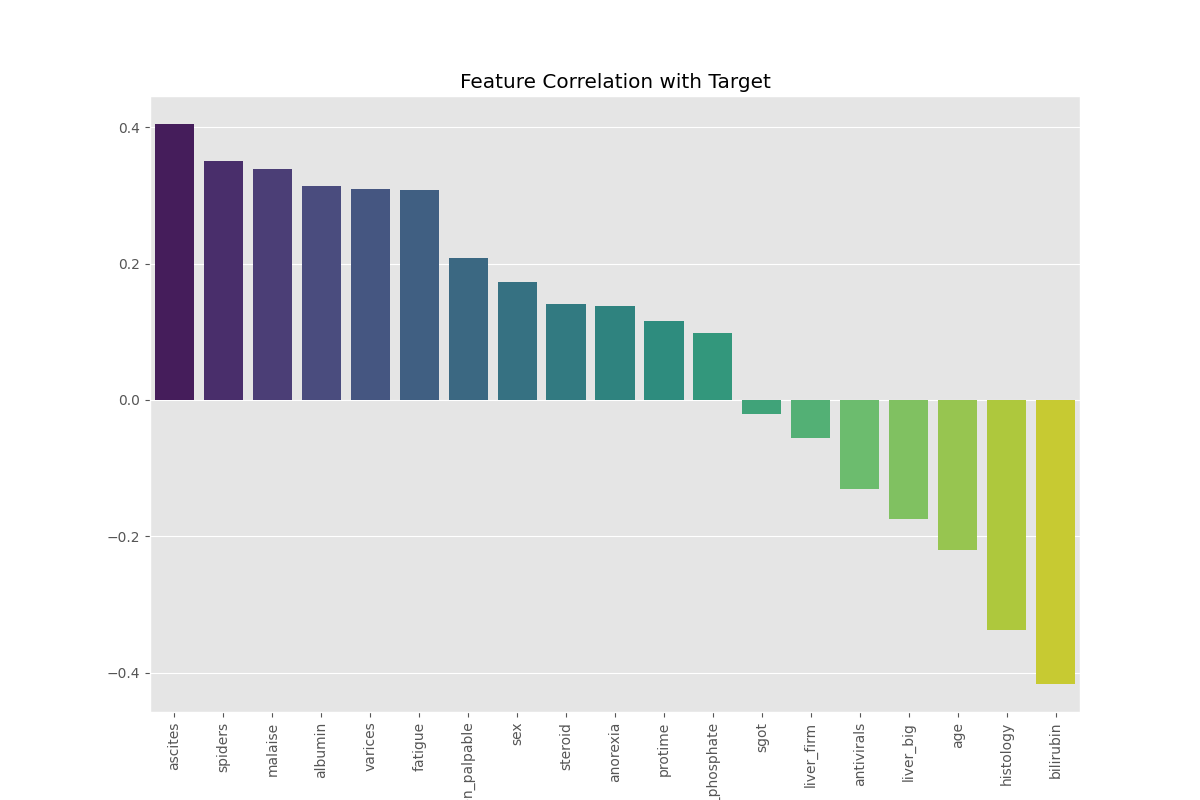
\includegraphics[width=0.75\textwidth]{../preprocessing/feature_correlation.png}}
  \caption{Correlation plot of all the variables with regards to the target variable.}
  \label{fig:corr}
\end{figure}

As can be seen, the correlation plots exhibit a well-balanced feature selection where some features negatively correlate with the target variable, whereas others positively correlate to the target variable. Due to the stochastic nature of Genetic Programming, this helped with convergence.

\section{GP Runtime Performance}
To improve the performance of the GP during runtime, C++'s pass by reference ability was utilised throughout the codebase to further improve performance. Because of the small dataset, no other optimisations have been done.

\section{GP Technical Specification}
\subsection{GP Setup}
Both the SBGP and the NGP followed the same setup apart from small alterations in some parts of the setup when needed for the SBGP. This allowed to work from the same GP implementation, reducing the overall code footprint.
\subsubsection{Control Model}
\label{steadyState}
To control the population of both the NGP and SBGP, a \textbf{steady-state control model (SSCM)} has been employed:
\begin{table}[H]
\centering
\begin{tabularx}{\textwidth}{X}
\hline
\begin{enumerate}[label=\arabic*.]
  \item Generate initial population
  \item Repeat \emph{until termination criteria is met}
  \begin{enumerate}[label*=\arabic*.]
    \item Tournament selection (winners)
    \item Inverse tournament selection (losers)
    \item Generate offspring by applying genetic operators to winners
    \item Replace losers with offspring
  \end{enumerate}
\end{enumerate} \\
\hline
\end{tabularx}
\end{table}

With SSCM, a fixed population size is maintained throughout the run where the offspring replaces individuals with poor fitness. The method to select the worst individuals is described in Section \ref{selection}. By replacing the worst individuals, top-performing individuals are preserved. This helps with steady convergence. On the other hand, a generational control model could potentially disrupt those individuals if no mechanism is put in place.

\subsubsection{Structure-based GP (SBGP) Specification}
To implement SBGP, a similar approach has been followed to ISBGP-II, as proposed by Kapoor and Pillay \cite{kapoor_genetic_2024}. This specific structure-based approach employs global and local similarity indices to adjust the search strategy. Global search allows for wider exploration, while the indication of a promising individual further exploits the program. Once local search fails it returns to global search. This essentially escapes local optima. The SSCM model (Section \ref{steadyState}) is modified for SBGP as follows:
\begin{table}[H]
\centering
\begin{tabularx}{\textwidth}{X}
\hline
\begin{enumerate}[label=\arabic*.]
  \item Generate initial population
  \item \textbf{Enable global search}
  \item Repeat \emph{until termination criteria is met}
  \begin{enumerate}[label*=\arabic*.]
    \item Tournament selection (winners)
    \item Inverse tournament selection (losers)
    \item Generate offspring by applying genetic operators to winners
    \item \textbf{If global search is enabled}
    \begin{enumerate}[label*=\arabic*.]
      \item \textbf{Generate global index for offspring}
      \item \textbf{If index is below \texttt{globalThreshold}, replace losers with offspring and disable global search.} (we found a promising individual)
    \end{enumerate}
    \item \textbf{If global search is disabled} (i.e. local search)
    \begin{enumerate}[label*=\arabic*.]
      \item \textbf{Generate \underline{local} index for offspring}
      \item \textbf{If index is below \texttt{\underline{local}Threshold}, replace losers with offspring.} 
      \item \textbf{Otherwise enable global search} (we possibly reached a local optima)
    \end{enumerate}
  \end{enumerate}
\end{enumerate} \\
\hline
\end{tabularx}
\end{table}

\subsubsection{Representation}
The individuals in the population were represented as a tree. Each subtree can have up to two subtrees, where \texttt{children} denotes one or more subtrees. The functions (non-terminal nodes) were mathematical and/or logical operators and the terminals (terminal nodes) were features or real numbers. The output of the tree is first passed into a \texttt{tanh}-function before being converted to a binary number by means of a predefined threshold. If the tree happen to be invalid, it will bypass the fitness calculation (described in Section \ref{fitness}) and output the worst possible fitness, which is \texttt{0.0} in this case (0\% accuracy).

\subsubsection{Function and Terminal Set}
\texttt{randomTerminal()} and \texttt{randomOperator()} functions determined which terminal or operator is chosen when generating a tree. Arithmetic operators (\texttt{+,-,/,*}) helps to combine continuous features. Non-linear functions (\texttt{tanh,sin,cos,log}) allows to model non-linear interactions and helps with scaling values more or less between \(-2.0\) and \(2.0\). Conditional operators also helped with scaling (e.g. two values compared outputs either \(0.0\) or \(1.0\)) but also helped with \emph{routing} the output, such as when a subtree becomes irrelevant.
In terms of the terminal set, all variables were kept as they all influenced the target variable (Figure \ref{fig:corr}). \texttt{double} were also added, which helps with bias offset and scaling. The GP's function and terminal set:
\begin{verbatim}
  F = {+, -, /, *, max, min, tanh, sin, cos, log, 
      <, >, <=, >=, ==, !=}
  T = {double, age, sex, steroid, antivirals, fatigue,
    malaise, anorexia, liver_big, liver_firm,
    spleen_palpable, spiders, ascites, varices,
    bilirubin, alk_phosphate, sgot, albumin,
    protime, histology}
\end{verbatim}
where \texttt{double} is a random real number between -0.5 and 0.5. The features from the dataset differed between continuous and discrete variables, but could co-occur. Experimentation were done to separate continuous and discrete features, but it turned out that if the trees were discrete close to the root, it barely used continuous features elsewhere, causing the tree to be biased towards one class. Since the continuous variables are normalised between 0.0 and 1.0, it worked well with the discrete variables between 0.0 and 1.0.

\subsubsection{Train/test split}
A standard 80\%/20\% train split was used The datasets were shuffled before splitting them for training and testing to ensure randomness. This training split gave enough data to fit without leaving too little data for testing.

\subsubsection{Initial Population}
\label{initPop}
The initial population was generated using a randomised grow method with \texttt{maxDepth} as a generation-specific parameter.

For each iteration, two booleans would independently determine if a left or right subtree would be further generated or not. The chance of these two booleans being true is increasingly determined by the current \texttt{maxDepth}. In the recursive function, \texttt{maxDepth} decreases as the tree grows.

\subsubsection{Tournament Selection}
\label{selection}
For the selection method, a tried-and-trusted tournament selection has been used. This selection method selects \(n\) random candidates to potentially apply genetic operators to. The two candidates with the best fitness is selected as parents. If the mutation operator is applied, the best parent is selected. Intuitively, for crossover, both parents are passed as parameters, and for reproduction, the two parents are passed onto the next generation.

To select individuals with poor fitness, \textbf{inverse tournament selection} has also been employed to find the two worst candidates to be replaced with the offspring.

Tournament selection was chosen to offer a balance between exploitation and exploration. It's also computationally efficient, since only the fitness of a few individuals in the population have to be calculated.

\subsubsection{Mutation}
For the mutation genetic operator, a mix of approaches has been followed to ensure maximum diversity. A random point in the tree is chosen, and a random subtree (possibly just a leaf node) is generated and the subtree is replaced. This ensures that both grow and shrink mutation is possible with this approach. The mutation operator also employed point mutation (50\% chance), which replaced the node with a terminal or a function, depending on it's position.

The root node is also replacable, but because \texttt{rand() mod maxDepth} is passed as parameter, it becomes possible to penalise bigger trees, by generating a new smaller tree (i.e. the root is replaced by a smaller tree). Having a replacable root node is potentially harmful to the individual, but no notable problems have been picked up.

For SBGP, if the mutation point was above the cutoff depth during local search, mutation was skipped.

The combination of subtree and point mutation offers multiple ways to explore new regions. Mutation is a good genetic operator to bring in completely new elements to the program space.

\subsubsection{Crossover}
The crossover operator takes a standard approach by selecting random points in each of the two parents, and then swaps them around to produce offspring. The root nodes can't be swapped, because pointers would then be swopped, which caused upstream problems when replacing offspring with the losers.

For SBGP, if any of the crossover points were above the cutoff depth during local search, the crossover attempt was cancelled. However, a retry mechanism was added to attempt other points in the tree to apply crossover to.

Crossover offers the opportunity to swop partially good solutions with each other in the program space. Moreover, the offspring are generally fit as their parents are fit as well. Crossover is a good choice for protecting good solutions, and seeking a solution that is potentially better.

\subsubsection{Reproduction}
The selected individuals remains unchanged and is carried over to the next generation. In the codebase, the reproduction rate is calculated as \(1.0-C_r-M_r\) where \(C_r\) is crossover rate and \(M_r\) is mutation rate. Reproduction helps to preserve fit individuals.

\subsubsection{Stopping Criteria}
For the stopping criterion, every GP run completed the full amount of generations (i.e. \texttt{maxGenerations}). No experimentation with early stopping or convergence testing has been done in this assignment. The final result were used to understand where the best convergence point were for multiple generations. Experiments with different \texttt{maxGenerations} has been done to see which one performs best.

Fixing the number of generations ensures that runs can converge sufficiently, whereas early stopping could potentially accept an average solution over a better solution.

\subsection{Fitness Function: BACC}
\label{fitness}
To evaluate the performance of the GP, Balanced Accuracy (BACC) has been used as the \texttt{fitness()}-function. BACC works well for datasets that are imbalanced by making sure that both positive and negative classes are weighted equally. Sensitivity accounts for the positive classes whereas specificity caters for the negative classes. The average between these two are taken and is be defined as follows:
\begin{equation}\label{BACC}
  BACC = \frac{\text{specificity} + \text{sensitivity}}{2.0}
\end{equation}

where \(\text{specificity} = \frac{TN}{TN + FP}\) and \(\text{sensitivity} = \frac{TP}{TP + FN}\). If \(TP + FN = 0.0\) or \(TN + FP = 0.0\), a bad fitness of \(0.0\) was returned.

To ensure the threshold can be applied when calculating BACC, the \(tanh\) function was used to ensure the output resides around \(0.0\):
\begin{equation}\label{eq:sigmoid}
  f(x) = tanh(x)
\end{equation}
The \(tanh\) function ensures smooth, bounded outputs between -1.0 and 1.0, which improves numeric stability (no overflow/underflow).

Because the \(tanh\) function outputs continuous values, a clipping mechamism was used:
\begin{equation}
\text{clip}(x)=
    \begin{cases}
        1.0 & \text{if } x > \text{threshold}\\
        0.0 & \text{otherwise}
    \end{cases}
\end{equation}
where the threshold were set to 0.0. If the tree output was 0.0 (i.e. die) then \(tanh(0) = 0\). Before starting with optimising parameters, F1-score and normal accuracy have also been experimented with, as well as an upsampled dataset, but BACC with a normal dataset was chosen to balance the predictions.

\section{Parameters and Results}
\label{GPsetup}
The parameters were manually tuned to achieve optimal performance. A wide range of variables have been experimented with. Reasoning have been provided next to each parameter.

\subsection{NGP Parameters}
After fine-tuning the parameters, the following NGP parameter setup is used:
\begin{itemize}
  \item Population size: \textbf{35} \emph{(Greater population size led to increased runtime with minimal performance improvements.)}
  \item Number of generations: \textbf{70} \emph{(A greater number of generations led to increased runtime. The GP already converged and didn't notably impact the results.)}
  \item Crossover rate: \textbf{0.6} \emph{(Higher crossover rates reduced convergence. A reasonably low crossover rate helped for convergence.)}
  \item Mutation rate: \textbf{0.25} \emph{(A high mutation rate was selected to allow the model to naturally escape local optima.)}
  \item Reproduction rate: \textbf{0.15} \emph{(The reproduction rate was simply a fallback and simply transfers the parents to the next generation.)}
  \item Max Depth: \textbf{7} \emph{(The initial depth is set to cater for the amount of variables and allow for genetic diversity. Furthermore, this allowed trees to have a wider range of depths due to the initial population generation method described in Section \ref{initPop}.)} 
  \item Tournament Size: \textbf{7} \emph{(The tournament size was made quite big to explore a big search space (20\% of the population size).)}
  \item Run \(n\)'s seed \(i\) is \(i = n-1\). \emph{(This remained unchanged from the start.)}
\end{itemize}

\subsection{SBGP Parameters}
After fine-tuning the parameters, the following SBGP parameter setup is used:
\begin{itemize}
  \item Population size: \textbf{35} \emph{(Greater population size led to increased runtime with minimal performance improvements.)}
  \item Number of generations: \textbf{110} \emph{(More generations were required than the NGP, likely due to the application of the local and global threshold.)}
  \item Crossover rate: \textbf{0.5} \emph{(Crossover did not seem to help too much with the convergence, and was therefore kept on the low side. This value is mostly inspired by Kapoor and Pillay \cite{kapoor_genetic_2024}.)}
  \item Mutation rate: \textbf{0.25} \emph{(The mutation rate were set high to escape possible local optima and to allow solutions to be accepted. This allowed for genetic diversity throughout the run. This value is also inspired by Kapoor and Pillay \cite{kapoor_genetic_2024}.)}
  \item Reproduction rate: \textbf{0.25 }\emph{(The reproduction rate was simply a fallback and simply transfers the parents to the next generation.)}
  \item Max Depth: \textbf{6} \emph{(A smaller number than NGP's max depth was chosen to cater for the thresholding mechanism. There's a strong correlation between this parameter and the cutoff depth. This is not the strict max depth, but rather the initial max depth.)} 
  \item Tournament Size: \textbf{7} \emph{(The tournament size was made quite big to explore a big search space (20\% of the population size), which helped for exploration.)}
  \item Run \(n\)'s seed \(i\) is \(i = n-1\). \emph{(This remained unchanged from the start.)}
\end{itemize}
On top of that, specific SBGP parameters were added:
\begin{itemize}
  \item Local threshold: \textbf{8} \emph{(Manual tuning were done to find the best value for overall performance.)}
  \item Global threshold: \textbf{6} \emph{(Manual tuning were done to find the best value for overall performance.)}
  \item Cutoff Depth: \textbf{4} \emph{(Manual tuning were done to find the best value for overall performance. As mentioned before, this value is correlated with the initial maximum depth.)}
\end{itemize}

\subsection{Results}
\begin{figure}[H]
  \makebox[\textwidth][c]{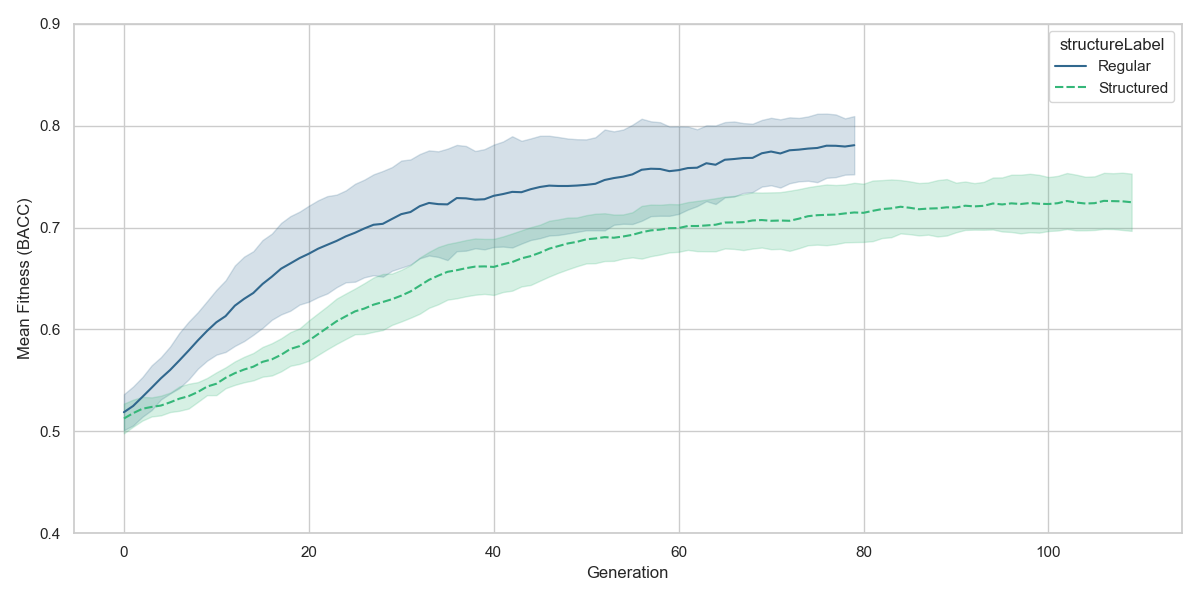
\includegraphics[width=1.1\textwidth]{assets/gpPopFitness.png}}
  \caption{Population fitness over multiple runs. It's evident in this figure that SBGP required more runs to converge whereas NGP runs converged sufficiently after 75 generations. NGP's runs were more stable, where SBGP likely depended more on whether to escape local optima.}
  \label{fig:gpPopResults}
\end{figure}

\begin{figure}[H]
  \makebox[\textwidth][c]{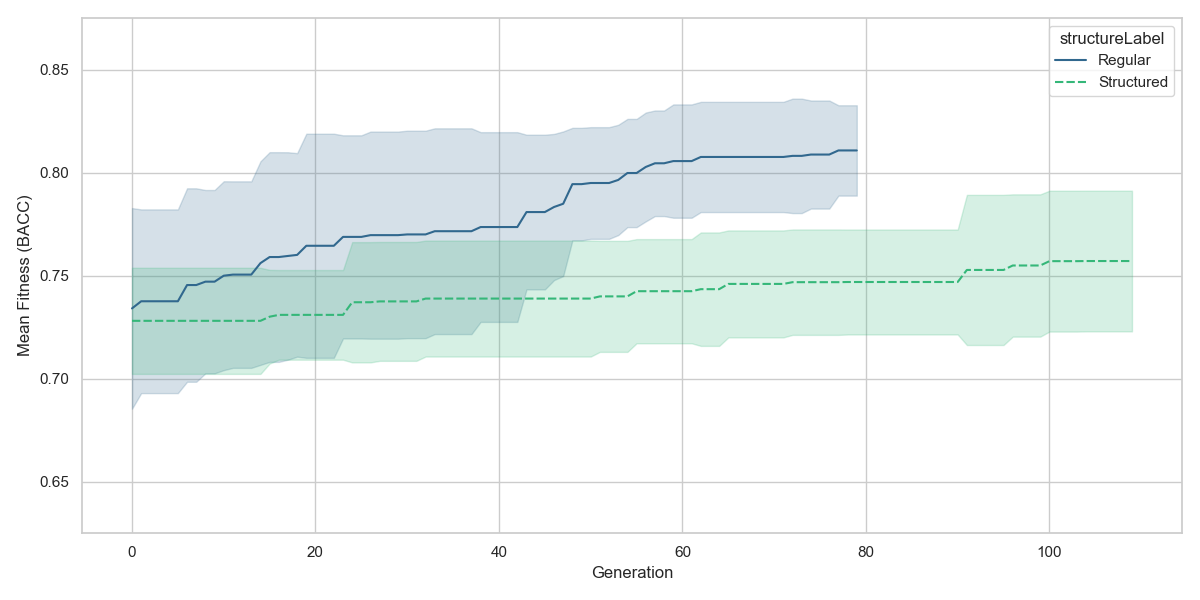
\includegraphics[width=1.1\textwidth]{assets/GPbest.png}}
  \caption{Progression of best tree fitness per generation for both the NGP and SBGP variants across all runs.}
  \label{fig:gpBestResults}
\end{figure}

\subsubsection{Training Results}
\begin{table}[H]
\centering
\resizebox{\textwidth}{!}{
\begin{tabular}{l|rrrr|rrrr}
\toprule
& \multicolumn{4}{l|}{\emph{Best Tree Statistics (BACC Fitness)}} & \multicolumn{4}{l}{\emph{Population Statistics (BACC Fitness)}} \\
Run & Mean & Min & Max & Std & Mean & Min & Max & Std \\
\midrule
0 & 0.803983 & 0.778367 & 0.822653 & 0.016623 & 0.739508 & 0.514927 & 0.814245 & 0.082290 \\
1 & 0.751166 & 0.669184 & 0.772449 & 0.025206 & 0.713052 & 0.529096 & 0.762163 & 0.064955 \\
2 & 0.796879 & 0.783460 & 0.798611 & 0.004855 & 0.743261 & 0.504960 & 0.798611 & 0.079888 \\
3 & 0.805149 & 0.757137 & 0.823751 & 0.023970 & 0.739562 & 0.542800 & 0.813062 & 0.072494 \\
4 & 0.738013 & 0.674060 & 0.743421 & 0.013222 & 0.690625 & 0.503136 & 0.743330 & 0.070118 \\
5 & 0.768891 & 0.747685 & 0.773727 & 0.010200 & 0.729921 & 0.539964 & 0.773727 & 0.060717 \\
6 & 0.784124 & 0.756970 & 0.795304 & 0.007241 & 0.732184 & 0.530353 & 0.784514 & 0.071208 \\
7 & 0.774320 & 0.674060 & 0.799248 & 0.035074 & 0.717953 & 0.520440 & 0.797385 & 0.077072 \\
8 & 0.776458 & 0.757143 & 0.782653 & 0.011018 & 0.728679 & 0.514070 & 0.782653 & 0.072485 \\
9 & 0.719593 & 0.714512 & 0.719667 & 0.000616 & 0.692540 & 0.549054 & 0.719667 & 0.038272 \\
\hline
\hline
Overall & \textbf{0.771858} & 0.669184 & 0.823751 & 0.028398 & 0.722728 & 0.503136 & 0.814245 & 0.018919 \\
\bottomrule
\end{tabular}}
\caption{\textbf{NGP Training Results:} Best Tree Fitness and Population Fitness statistics per GP run. The Overall row shows the mean across runs, the best result achieved in any run, the worst best result in any run, and the standard deviation of means across runs.}
\label{ngpResults}
\end{table}

\begin{table}[H]
\centering
\resizebox{\textwidth}{!}{
\begin{tabular}{l|rrrr|rrrr}
\toprule
& \multicolumn{4}{l|}{\emph{Best Tree Statistics (BACC Fitness)}} & \multicolumn{4}{l}{\emph{Population Statistics (BACC Fitness)}} \\
Run & Mean & Min & Max & Std & Mean & Min & Max & Std \\
\midrule
0 & 0.733725 & 0.690000 & 0.782245 & 0.035523 & 0.631417 & 0.485516 & 0.744023 & 0.082394 \\
1 & 0.730408 & 0.730408 & 0.730408 & 0.000000 & 0.692305 & 0.527819 & 0.730408 & 0.056291 \\
2 & 0.726601 & 0.717803 & 0.763889 & 0.018196 & 0.639497 & 0.515711 & 0.739412 & 0.057466 \\
3 & 0.752511 & 0.686360 & 0.774980 & 0.022280 & 0.712234 & 0.525382 & 0.774980 & 0.066870 \\
4 & 0.740138 & 0.676128 & 0.761090 & 0.035194 & 0.703818 & 0.508002 & 0.761090 & 0.070182 \\
5 & 0.761458 & 0.690972 & 0.782407 & 0.021149 & 0.723699 & 0.511541 & 0.776141 & 0.067833 \\
6 & 0.741031 & 0.725055 & 0.742480 & 0.004538 & 0.705974 & 0.516754 & 0.742480 & 0.053186 \\
7 & 0.740432 & 0.701316 & 0.777068 & 0.029074 & 0.709218 & 0.528958 & 0.774060 & 0.059437 \\
8 & 0.775965 & 0.742653 & 0.777551 & 0.007302 & 0.747951 & 0.510391 & 0.777551 & 0.063148 \\
9 & 0.767915 & 0.716891 & 0.775971 & 0.020368 & 0.730369 & 0.498425 & 0.775971 & 0.076455 \\
\hline
\hline
Overall & \textbf{0.747018} & 0.676128 & 0.782407 & 0.016697 & 0.699648 & 0.485516 & 0.777551 & 0.037253 \\
\bottomrule
\end{tabular}}
\caption{\textbf{SBGP Training Results:} Best Tree Fitness and Population Fitness statistics per SBGP run. The Overall row shows the mean across runs, the best result achieved in any run, the worst best result in any run, and the standard deviation of means across runs.}
\label{sbgpResults}
\end{table}

\subsubsection{Testing Results}
\begin{table}[H]
\centering
\begin{tabular}{cccc}
\toprule
\textbf{Run} & \textbf{NGP} & \textbf{SBGP} & \textbf{Difference} \\
\midrule
1  & 0.711310 & \textbf{0.782738} & +0.071428 \\
2  & \textbf{0.803571} & 0.729167 & $-$0.074404 \\
3  & 0.660326 & \textbf{0.785326} & +0.125000 \\
4  & 0.673333 & \textbf{0.796667} & +0.123334 \\
5  & \textbf{0.907407} & 0.708333 & $-$0.199074 \\
6  & 0.761538 & \textbf{0.884615} & +0.123077 \\
7  & 0.750000 & \textbf{0.892857} & +0.142857 \\
8  & 0.638889 & \textbf{0.833333} & +0.194444 \\
9  & 0.732143 & \textbf{0.782738} & +0.050595 \\
10 & 0.590000 & \textbf{0.656667} & +0.066667 \\
\midrule
Average & 0.722852 & \textbf{0.785244} & +0.062392 \\
\bottomrule
\end{tabular}
\caption{\textbf{Test Results:} Comparison of NGP and SBGP fitness (BACC) across 10 runs. Positive differences indicate better performance by SBGP.}
\label{tab:bacc_comparison}
\end{table}

\section{Discussion}
SBGP is an interesting avenue to build and train a GP model for data classification. Different than a normal GP implementation, SBGP attempts to control the search space, but comes with a number of challenges. During experimentation, as seen in Figure \ref{fig:gpPopResults} and Figure \ref{fig:gpBestResults}, it is noted that the SBGP required more generations to converge similarly to the baseline GP (NGP). This is likely due to the \emph{gating} that the local and global threshold employs, where some good-enough solutions might be rejected due to possible local optima.

Even though NGP converged, there were signs of overfitting as the training accuracy were lower than the testing accuracy. However, with the SBGP, underfitting is noted since the mean test accuracy is higher than the mean train accuracy. The case for underfitting could likely be traced back to the dataset being relatively small.

In both cases, the mechanisms employed in the fitness function played an important role to accurately measure the outcomes of the individuals. It's also observed in Table \ref{ngpResults} and Table \ref{sbgpResults} that SBGP's population's standard deviation is almost double NGP's standard deviation, indicating better diversity and exploration.

With the aim of maximising BACC, SBGP outperforms the NGP on testing data by 6.24\% (Table \ref{tab:bacc_comparison}). However, the SBGP struggled when the parameters were not tuned well, and it's likely that there are better parameters for this specific solution. Further work could include a more fine-grained approach to determining exact function and terminal sets. Due to time constraints, no automated parameter fine-tuning methods were explored, which could potentially improve the overall solution. Another addition could be to threshold continuous variables to act as boolean variables, but is not guaranteed to work. Other genetic operators such as the edit operator could also help to identify individuals with local optima and replace nodes in the individual tree with better nodes. This is not necessarily meant to directly improve fitness, but rather to ensure genetic diversity and mitigate local optima. Data scarcity was a problem in this assignment, and preprocessing techniques such as upsampling can be explored to potentially expose better performance.

In conclusion, SBGP is not domain-specific and can readily be adapted to other domains and datasets with sufficient parameter fine-tuning and GP setup. It is shown in this report that by controlling the search space, performance increases can be observed.

\bibliographystyle{IEEEtran}
\bibliography{COS710A1}

\end{document}
